
%%%%%%%%%%%%%%%%%%%%%%%%
%% ObjectManipulation %%
%%%%%%%%%%%%%%%%%%%%%%%%

\section{Object Manipulation} 

\subsection{Description}

In the object manipulation scenario, there are two types of objects scattered throughout the environment, objects for collection and object for destruction.  Thus, the swarm has two simultaneous goals: (1) locate all collectible objects and return them to a defined goal location and (2) locate and destroy all objects marked for destruction.  

Object manipulation presents many interesting challenges for a swarm.  Different types of coordination are required to address each of the separate tasks, these being collection and destruction.  Object collection requires the development of a primarily independent agent strategy.  Though the agents can interact by communicating the location of an object, the actual act of collecting an object can only be performed by a single agent.  On the other hand, object destruction requires the development of a cooperative strategy because the destruction of an object is a multi-step process and whenever an agent completes one of those steps they become disabled.   From a theoretical perspective, object manipulation is interesting because there is not a trivial solution.  There are many different approaches that may be taken to address the object manipulation problem, and thus providing an adequate final scenario to test the abilities of the evolutionary system developed in this work.

This section discusses the evolution of the basic object manipulation swarm algorithm.  A three phase approach will be taken for the evolution of an object manipulation algorithm.  First, the evolution of an object collection algorithm and an object destruction algorithm will be addressed separately.  Even though both are similar, there are salient features of each problem that will need to be accounted for separately.  Then, leveraging the work from evolving the object collection and destruction algorithms, an algorithm for the full object manipulation problem will be undertaken.
 
%% ObjectManipulation->Implementation
\subsection{Implementation}

This section will separately discuss the implementation details used for both the object collection and object destruction scenarios.  It is assumed that the object manipulation scenario will use the combined implementations for object collection and destruction.

\subsubsection{Scenario Description}

There are two types of objects randomly scattered throughout the environment, objects to be collected (type $C$) and objects to be destroyed (type $D$).  The type $C$ objects are to be located and returned to a predisposed goal repository known to all the agents.  The type $D$ objects require two separate \qw{attacks} to be completely destroyed.  As a by-product of an agent attacking an object, that agent is disabled for the duration of the simulation.  Type $D$ objects have three distinct states: untouched, damaged, and destroyed.  All type $D$ objects originate in the untouched state, and must become damaged before they are destroyed.  When an agent first attacks an object, the object transitions from the untouched to the damaged state.  When another agent attacks an object in the damaged state, the object transitions to the destroyed state.

The agents in this scenario are free-moving and have the ability to randomly wander.  The initial physical configuration of the swarm is arbitrary, thus a random distribution through the environment is assumed.  An agent is able to sense and differentiate between type $C$ and $D$ objects.  Additionally, the ability to navigate directly towards an object is incorporated to eliminate the need to evolve path planning capabilities, which is beyond the scope of this work.  Finally, an agent has the ability to distinctly broadcast to near-by neighbors the location of sensed objects.  When an agent receives a broadcast, the information is treated similarly to that of the object proximity sensor, thus the broadcasted information is compatible with the navigation behaviors.

\subsubsection{Agent Behaviors}

\refTable{ObjectActions} and \refTable{ObjectSensors} provide a summary of the actions and sensors available as state machine building blocks.  For both cases, the default behavior when no transition fires is \emph{move-random}.  Additionally, each agent is equipped with one sensor that indicates when the agent is on an object, and one sensor that indicates when the agent is near an object.  With the implementation used in this work, when an agent is on an object, the agent is also considered near an object.

The basic agent behaviors related to movement are \emph{move-up}, \emph{move-down}, \emph{move-left}, \emph{move-right}, and \emph{move-random}.  Since the focus of this work is the evolution of high-level algorithms, utility \emph{move-to} behaviors are also provided to navigate an agent to certain locations.  Specifically, the \emph{move-to-goal} behavior navigates the agent to the known goal location, while \emph{move-to-object\_C} and \emph{move-to-object\_D} navigates an agent toward the nearest type $C$ or $D$ object, respectively.  

The \emph{pick-up} and \emph{put-down} behaviors are used to interact with type $C$ objects.  An agent can only pick up a type $C$ object when they are physically on top of the object, and an object can only be put down when the agent is in the goal area.  The \emph{first-attack} and \emph{second-attack} behaviors are used to interact with type $D$ objects.  Each type $D$ object requires two separate \qw{attacks} to be completely destroyed.  Each agent has the ability to execute either attack action.  Additionally, a side-effect of each attack is that upon a successful attack, the performing agent becomes disabled for the duration of the simulation.  Note, a minimum of $2n$ agents are required to destroy $n$ type $D$ objects.

Finally, agents can communicate through the \emph{broadcast\_C} and \emph{broadcast\_D} behaviors, which broadcast to agents in a defined range the location of the nearest type $C$ or $D$ object, respectively.

\subsubsection{Agent Sensors}

Each agent has a number of proximity sensors that provide them with information about their environment.  Two basic classes of sensors are defined, \emph{near} and \emph{on}.  A \emph{near} sensor returns \true{} when an agent is within a defined range of some object, whereas an \emph{on} sensor will only return \true{} when an agent is physically on some object.  Note that with this implementation, when an agent is \qw{on} an object, they are also \qw{near} that same object.  Thus,  a rule $r_1$ using an \emph{on} sensor as input should be ordered before a rule $r_2$ using a \emph{near} sensor so as to ensure that $r_1$ is evaluated.  In total, six sensors are defined: \emph{near-object\_C}, \emph{near-object\_D}, \emph{on-object\_C}, \emph{on-object\_D(untouched)}, \emph{on-object\_D(damaged)}, and \emph{on-goal}.  The two different \emph{on} sensors for type $D$ objects allow the agent to differentiate between untouched and partially destroyed objects, and hence differentiate when to use \emph{first-attack} and \emph{second-attack}.


\begin{table}[ht]
  \centering
    \begin{tabular}{|l||c|c|c|}
      \hline
      \multirow{2}{*}{\textbf{Behavior}} & \multicolumn{3}{c|}{\textbf{Scenarios}}  \\
       & Collection & Destruction & Manipulation \\
      \hline
      \hline
      \emph{move-up}           & x & x & x \\
      \emph{move-down}         & x & x & x \\
      \emph{move-left}         & x & x & x \\
      \emph{move-right}        & x & x & x \\
      \emph{move-random}       & x & x & x \\
      \hline
      \emph{pick-up}           & x &   & x \\
      \emph{put-down}          & x &   & x \\
      \emph{move-to-goal}      & x &   & x \\
      \emph{broadcast\_C}      & x &   & x \\
      \emph{move-to-object\_C} & x &   & x \\
      \hline
      \emph{first-attack}      &   & x & x \\
      \emph{second-attack}     &   & x & x \\
      \emph{broadcast\_D}      &   & x & x \\ 
      \emph{move-to-object\_D} &   & x & x \\
      \hline
    \end{tabular}
	\caption{Object manipulation behavior primitives available for state machine construction.}
    \label{tab:ObjectActions}
\end{table}

\begin{table}[ht]
  \centering
  \begin{tabular}{|l||c|c|c|}
    \hline
	\multirow{2}{*}{\textbf{Sensor}} & \multicolumn{3}{c|}{\textbf{Scenarios}}  \\
       & Collection & Destruction & Manipulation \\
    \hline
    \hline
    \emph{near-object\_C}          & x &   & x \\
    \emph{on-object\_C}            & x &   & x \\
    \emph{holding-object\_C}       & x &   & x \\
    \emph{on-goal}                 & x &   & x \\
    \hline
    \emph{near-object\_D}          &   & x & x \\
    \emph{on-object\_D(untouched)} &   & x & x \\
    \emph{on-object\_D(damaged)}   &   & x & x \\
    \hline
  \end{tabular}
  \caption{Object manipulation sensor primitives available for constructing state transitions.}
  \label{tab:ObjectSensors}
\end{table}

\subsubsection{Fitness Metrics}

\refTable{ObjectMetrics} describes the raw metrics that evaluate the performance of a candidate solution with regards to the object collection and object destruction scenarios.  The metrics are formulated in terms of how much of a task is performed, thus the overall goal is to maximize the fitness measures.  Additionally, all metrics are evaluated on the final timestep of the \SWEEP{} simulation used to generate the raw fitness data.

\begin{table}[ht]
  \centering
  \begin{tabular}{|c|l|}
    \hline
    Name & Description \\
    \hline
    $c_{1}$ & number of objects put in the goal      \\
    $c_{2}$ & number of objects picked-up            \\
    $d_{1}$ & number of objects completely destroyed \\
    $d_{2}$ & number of objects partially destrroyed \\
    $t$     & normalized execution speed             \\
    \hline
  \end{tabular}
  
\caption{Basic fitness metrics for an object manipulation scenario.}
\label{tab:ObjectMetrics}
\end{table}

The metric $t$ measures the normalized execution speed of an evolved candidate algorithm in terms of simulation timesteps.  Given the maximum execution time as 400 timesteps (\refTable{ManipulationParameters}), and $t_{actual}$ as the measured length of the simulation in timesteps, then $t=1-\frac{t_{actual}}{400}$.  The metric $t$ will have a value of 0 when a simulation exceeds the maximum execution time.  Thus, larger values of $t$ indicate that the evolved algorithm is executing faster.  

Two metrics are defined to measure the fitness of a candidate object collection algorithm.  As described in \refTable{ObjectMetrics}, metric $c_2$ measures the number of objects picked-up, and metric $c_1$ measures the number of object picked-up and returned to the repository.  For the individual solution fitness scores, the metrics are ordered in decreasing importance: $c_1$, $c_2$, $t$.

Similarly, two metrics are defined to measure the fitness of a candidate object destruction algorithm.  As shown in \refTable{ObjectMetrics}, metric $d_2$ measures the number of partially destroyed objects, and metric $d_1$ measures the number of completely destroyed objects.  For the individual solution fitness scores, the metrics are ordered in decreasing importance: $d_1$, $d_2$, $t$.  

As seen in the object collection and object destruction fitness metrics, the ordering of the metrics also coincides with the sequential dependencies inherent in the scenario.  In the object manipulation scenario, the sequential dependency problem becomes more pronounced as the sequential dependencies that exist for the individual object collection and destruction subtasks are independent but equally weighted.  Since $c_1$ and $d_1$ are equally weighted, the ordering of the two metrics skews the evolutionary progress towards the metric given sequential preference.  For example, when $c_1$ is given preference over $d_1$, the solution pool tends to first evolve experts in object collection, then the system has to modify through mutation an expert object collection algorithm to accommodate for object destruction \cite{kovacina:AdaptiveIntelligentEvolution}.

Since $c_1$ and $d_1$, and $c_2$ and $d_2$, are independent but equally weighted, a regular ordering is not enough to adequately characterize the object manipulation scenario.  Thus, to address this issue, the raw fitness metrics are used to construct a set of composite metrics that do not exhibit the sequentiality conflicts seen between the raw metrics.  \refTable{ManipulationMetrics} describes these composite metrics.  The use of these composite metrics enables the use of a radix sort to establish a fitness-based ordering.  The standard radix sort~\cite{clr} moves from the least significant position to the most significant position, resulting in a sorted list.  For this work, the most significant metric is $m_1$ and proceeds to the least significant metric, $m_8$.  For boolean metrics ($m_1$--$m_4$), \true{} is deemed greater than \false{}.  \refFigure{LexEx} shows a simple example of how radix sorting would be applied to a small population of solutions (more fit solutions at the top).

\begin{figure}[ht]
	\centering
	\begin{tabular}{c|c}

		\emph{Unsorted} & \emph{Sorted} \\
		\hline
		\{ true  5 3 9 \} & \{ true  8 3 6 \} \\
		\{ true  8 1 6 \} & \{ true  5 3 9 \} \\
		\{ false 4 2 7 \} & \{ true  5 3 3 \} \\
		\{ true  5 3 3 \} & \{ false 4 2 7 \} \\

	\end{tabular}
\caption[A simple example of radix sorting.]{A simple example of radix sorting.  Note that \true{} is deemed greater than \false{}, and that the solutions are sorted from most to least fit.}
\label{fig:LexEx}
\end{figure}

\begin{table}[ht]
  \centering
  {
  \small
  \begin{tabular}{|c|c|l|}
    \hline
    Name/Priority & Metric & Description \\
    \hline
    $m_1$ & $c_1 \wedge d_1$ & flag solutions fully performing both subgoals              \\
    $m_2$ & $c_2 \wedge d_2$ & flag solutions partially performing both subgoals          \\
    $m_3$ & $c_1 \vee d_1$   & flag solutions fully performing either subgoal             \\
    $m_4$ & $c_2 \vee d_2$   & flag solutions partially performing either subgoal         \\
    $m_5$ & $\min(c_1,d_1)$  & select the weakest of the two primary subgoals             \\
    $m_6$ & $\min(c_2,d_2)$  & select the weakest of the two secondary subgoals           \\
    $m_7$ & $\max(c_1,d_1)$  & select the strongest of the two primary subgoals           \\
    $m_8$ & $\max(c_2,d_2)$  & select the strongest of the two secondary subgoals         \\
    $m_9$ & $1-t_{actual}/t_{max}$ & normalized execution speed      \\
    \hline
  \end{tabular}
  }
  \caption[Composite metrics used for the object manipulation scenario.]{Composite metrics used for the object manipulation scenario.  The metrics are created from raw fitness data in order to eliminate the conflicting sequential dependencies that exist in using the raw fitness metrics.  Note, the value of $t_{max}$ is 400 timesteps (\refTable{ManipulationParameters}), and $t_{actual}$ is the candidate solution's execution speed in timesteps.}
  \label{tab:ManipulationMetrics}
\end{table}


In order to create the correct ordering needed for the object manipulation scenario, first a series of boolean flags are defined.  These flags ensure that the solutions that meet the flag criteria are ranked higher than those that do not.   Thus, higher-level logic can be incorporated into the radix scoring, such as the metrics $m_1$ and $m_2$ which encode the rule \qw{solutions that act on both subgoals are better than solutions that address only one subgoal.}  Metric $m_3$ ensures that a solution that completely addresses one subgoal is ranked higher than a solution that only partially addresses a subgoal, regardless of the raw metric values.  Metric $m_4$ ensures that solutions that partially address any subgoal are ranked higher than solutions that do nothing.  Though $m_4$ is not needed, it is included for completeness. Metrics $m_5$ and $m_6$ rank solutions according to their weakest subgoals, focusing on $c_1$/$d_1$ first and then $c_2$/$d_2$.  These metrics are implemented in this fashion because a solution's total fitness is only as good as the weakest component.  Similarly, metrics $m_7$ and $m_8$ rank solutions according to their strongest subgoals, focusing on $c_1$/$d_1$ first and then $c_2$/$d_2$.

\refTable{ManipulationParameters} summarizes the parameters used in the evolution of solutions for object collection, destruction, and manipulation.  All randomized operations (\ie{} solution generation, mutations, \ldots\@) use a random number generator with a uniform distribution.  All randomly generated solutions are created with exactly one state $s$ and one transition $t$.  All transitions are generated by randomly assigning a start state and a next-state from the solution's set of states.  For randomly generated solutions, the state $s$ is both the start state and next-state for the transition $t$.  The sensor condition and action associated with a transition are randomly selected from the solutions's set of sensor conditions and actions, respectively.  

Each of the five mutations are applied to eight solutions (the best 6 plus two selected from random) per generation.  Mutations are applied to a copy of the selected solution, the copy is evaluated using \SWEEP{}, and is then rolled back into the main population.  Thus, after all mutations are complete, the effective population size will be 72 (the original 32 plus 40 mutated).  Additionally, a single randomly generated solution is introduced into the population at each generation.

Each solution is evaluated using \SWEEP{}.  Fitness data from each solution is collected from \SWEEP over 2 different trials.  The data from all the trials is then combined to give an accumulated set of raw fitness data which is then passed to the fitness function.

\begin{table}[ht]
  \centering
  \small
  \begin{tabular}{|lc|}
    \hline
    \multicolumn{2}{|c|}{\em{Parameters}} \\
    Objective & Object Manipulation \\
    Max. Generations & 1000 \\
    Population Size & 32 \\
    Number of Trials & 2 \\
    \hline
    \hline
    \multicolumn{2}{|c|}{\em{Mutations}} \\
    Change-Sensor-Value & best 6 + 2 random \\
    Change-Action-Value & best 6 + 2 random \\
    Change-Next-State   & best 6 + 2 random \\
    Add-State           & best 6 + 2 random \\
    Add-Transition      & best 6 + 2 random \\
    \hline
    \hline
    \multicolumn{2}{|c|}{\em{Actions}} \\
    move-random         & move-to-object\_C   \\
    move-to-goal        & move-to-object\_D   \\
    pick-up             & put-down            \\
    first-attack        & second-attack       \\
    broadcast-object\_C & broadcast-object\_D \\
    \hline
    \multicolumn{2}{|c|}{\em{Sensors}} \\
    on-object\_C            & near-object\_C        \\
    on-goal                 & holding-object\_C     \\
    on-object\_D(untouched) & on-object\_D(damaged) \\
    \multicolumn{2}{|c|}{near-object\_D}            \\
    \hline
    \hline
    \multicolumn{2}{|c|}{\em{Simulation}} \\
    Number of Agents & 100 \\
    Environment & $50 \times 50$ grid \\
    Maximum time ($t_{max}$) & 400 \\
    Number objects type $C$ & 50 \\
    Number objects type $D$ & 30 \\
    Broadcast range & 25 \\
    Sensing range & 5 \\
    \hline 
  \end{tabular}
\caption{Parameters for evolving object collection, destruction, and manipulation}
\label{tab:ManipulationParameters}
\end{table}

\clearpage

\subsection{Results}

Viable solutions to each of the three scenarios outlined were successfully evolved.  The performance for the object destruction and object collection  scenarios were similar, with each finding a solution that completely addresses the secondary subgoal for the scenario.  Then, within 25 generations a complete solution is found, with a somewhat time optimized solution being evolved within 20 generations after that.  The object manipulation scenario has a longer convergence time, taking at least 300 generations to evolve a full solution, and up to 40 more generations to evolve a more time efficient solution.

The object destruction and object collection scenarios each had similar average convergence times, with object destruction being the slightly easier of the two scenarios.  From a practical standpoint, the object destruction scenario is the easiest of the three scenarios because the sequential subtasks are assigned to the swarm, not an individual agent.  Specifically unlike the object collection scenario where a single agent is responsible for both picking up and depositing an object, an agent in the object destruction scenario is only responsible for one \qw{attack} on an object, relying on another member of the swarm to complete the job.  Thus, evolution of object destruction behaviors is easier because the sequential dependencies on a single agent are eliminated. 

Separately looking at the average convergence times for the collection and destruction tasks in the object manipulation scenario (\refFigure{ManipulationBest} and \refFigure{ManipulationBest2}), the same convergence rate is not observed as when  the tasks are evolved separately (\refFigure{DestructionBest} and \refFigure{CollectionBest}).  This performance decrease is expected, as the collection and destruction tasks are in direct competition for the same pool of fitness resources.  So, the evolution of both behaviors simultaneously increases the competition faced by each solution at every generation.  In the early implementations of the system, this competition actually inhibited convergence because the the fitness function used a more traditional approach of weighting individual metrics, which led to the development of \qw{expert} solutions \cite{kovacina:AdaptiveIntelligentEvolution}.  In this case, an expert solution is one that is able to completely satisfy one goal but not the other, such as collecting all type $C$ objects but not destroying any type $D$ objects.  These expert solutions dominated the population, thus eventually they dominated reproduction, resulting in an almost homogeneous population.  Once the population was mostly homogenized, the system then focused on using mutations to transform an expert solution into a solution that addressed both goals.  The homogenization identified a need for a method to balance the evolution between multiple objectives, hence the introduction of the radix ranking method.  As seen in \refFigure{ManipulationBest} and \refFigure{ManipulationMean}, the radix ranking is able to balance the evolution towards both collection and destruction.  The simultaneous progress is made on each secondary subgoal, $m_6$ and $m_8$, and each primary subgoal, $m_5$ and $m_7$, thus enabling the simultaneous evolution of a complete solution for the object manipulation scenario.

\subsubsection{Object Destruction}

The average number of generations required to evolve a solution for object destruction is approximately 50 generations. As seen in \refFigure{DestructionBest}, within 2 generations a solution is found that completely maximizes $d_2$, and within 5 generations most of the population is able to almost maximize $d_2$, as shown by the mean fitness in \refFigure{DestructionMean}.  As the population drives towards maximizing $d_2$, slow progress is eventually made towards the maximization of $d_1$.  Mutated solutions that begin to maximize $d_1$ rise to the top of the fitness scale, thus being selected more often for reproduction.  Eventually in generation 14, a solution is produced that completely maximized $d_1$ and $d_2$.  As the population converges towards a set of complete solutions, the last metric to be addressed is the time $t$.  It is interesting to note how the mean fitness for the population decreases once a complete solution is found.  This behavior can be attributed to the mutations being applied during reproduction since at this point most of the solutions in the population maximize $d_1$ and $d_2$, thus the probability that a random mutation will be helpful is small.

A solution that completely maximizes both $d_1$ and $d_2$ is found in generation 14, but approximately 5 more generations of evolution is able to produce a solution that executes quickly.  The solution evolved here, shown in \refTable{DestructionAlgorithm}, is able to completely destroy all 30 objects in approximately 30 timesteps.  \refTable{DestructionAlgorithmReduced} is a simplified version of the evolved object destruction algorithm shown in \refTable{DestructionAlgorithm}.  The simplifications include the removal of unreachable states and non-firing transitions, and the removal of actions that will have no effect.  

Every agent executing the algorithm in \refTable{DestructionAlgorithmReduced} starts in state $A$.  If the agent is on any type $D$ object, the appropriate attack will be executed and the agent will be disabled for the duration of the simulation.  If the agent is not on a type $D$ object, the agent transitions to state $E$, where they will randomly wander until they are within sensing range of a type $D$ object.  Though unlikely here, if the agent stumbles upon a partially destroyed type $D$ object, they will attack it appropriately and become disabled.  What is more likely to happen that the agent will come in proximity to a type $D$ object, and since they are not on a partially destroyed type $D$ object, they will move towards the nearest type $D$ object and transition from state $E$ to $C$.   Implicit in the transitions from state $E$ to state $C$ is that the agent is near a type $D$ object, thus in state $C$ the first transition fires, moving an agent towards a type $D$ object and transitioning back to state $A$, where this cycle repeats until all the type $D$ objects are destroyed.    

The transition from state $E$ to state $C$ has the implied condition that the agent is near a type $D$ object, say \textit{$X$}, but since there are multiple agents executing this same algorithm, a race condition occurs.  It is conceivable that in the transition from $E$ to $C$ another agent completes the destruction \textit{$X$}, which will probably cause the agent that transitioned from $E$ to $C$ to execute the second transition in state $C$, sending the agent to state $J$.  In state $J$, the agent will randomly wander until it is sitting on top of an untouched type $D$ object, say \textit{$Y$}, at which time it will wander off \textit{$Y$} and transition to state $F$.  In the unlikely event that the agent wanders onto a partially destroyed type $D$ object, the second transition in state $F$ will fire, completing the destruction of a type $D$ object and disabling the agent.  More often though, the agent will execute the first transition in state $F$, bringing the agent back on top of \textit{$Y$} and causing a transition to state $H$, where the agent will enter a do-nothing infinite loop between states $H$ and $D$.  Only once another agent attacks \textit{$Y$} will the agent be able to break from the infinite loop.  In the end though, even if the agent is broken free from the $H$/$D$ infinite loop, the agent is relegated to transitioning between states $B$, $D$, $H$, and $I$ which do not provide much help in accomplishing the task of object destruction.

%The evolved solution takes advantage of the \emph{first-attack} and \emph{second-attack} implementations that only disable the agent when the behavior successfully destroys an object.  Thus, a typical agent following the algorithm outlined in \refTable{DestructionAlgorithmReduced} will continuously transition from $A \rightarrow F \rightarrow D \rightarrow A$ in order to move towards an object for an attack.  Untouched objects are acted on with \emph{first-attack} in state $A$, and damaged objects are acted upon in state $D$.  Embedded within that cycle at state $F$ is the execution of \emph{broadcast\_D}, which effectively informs nearby agent's that an object will soon be acted upon, and additional actions may be needed to completely destroy the object.  Thus, each agent broadcasting the location of an intended target object reduced the overall execution time for the scenario.

\begin{table}[ht]
  \centering
  \small
  \begin{tabular}{|c|c|p{25ex}|c|}
    \hline
    State & Condition & Action & Next State \\
    \hline
    \input{FSA/destruction.fsa}
  \end{tabular}
  \normalsize
  \caption{Evolved object destruction state machine}
  \label{tab:DestructionAlgorithm}
\end{table}

\begin{table}[ht]
  \centering
  \small
  \begin{tabular}{|c|c|p{25ex}|c|}
    \hline
    State & Condition & Action & Next State \\
    \hline
    \input{FSA/destruction-reduced.fsa}
  \end{tabular}
  \normalsize
  \caption{Simplified version of the evolved object destruction state machine}
  \label{tab:DestructionAlgorithmReduced}
\end{table}

\begin{figure}[f]
  \centering
  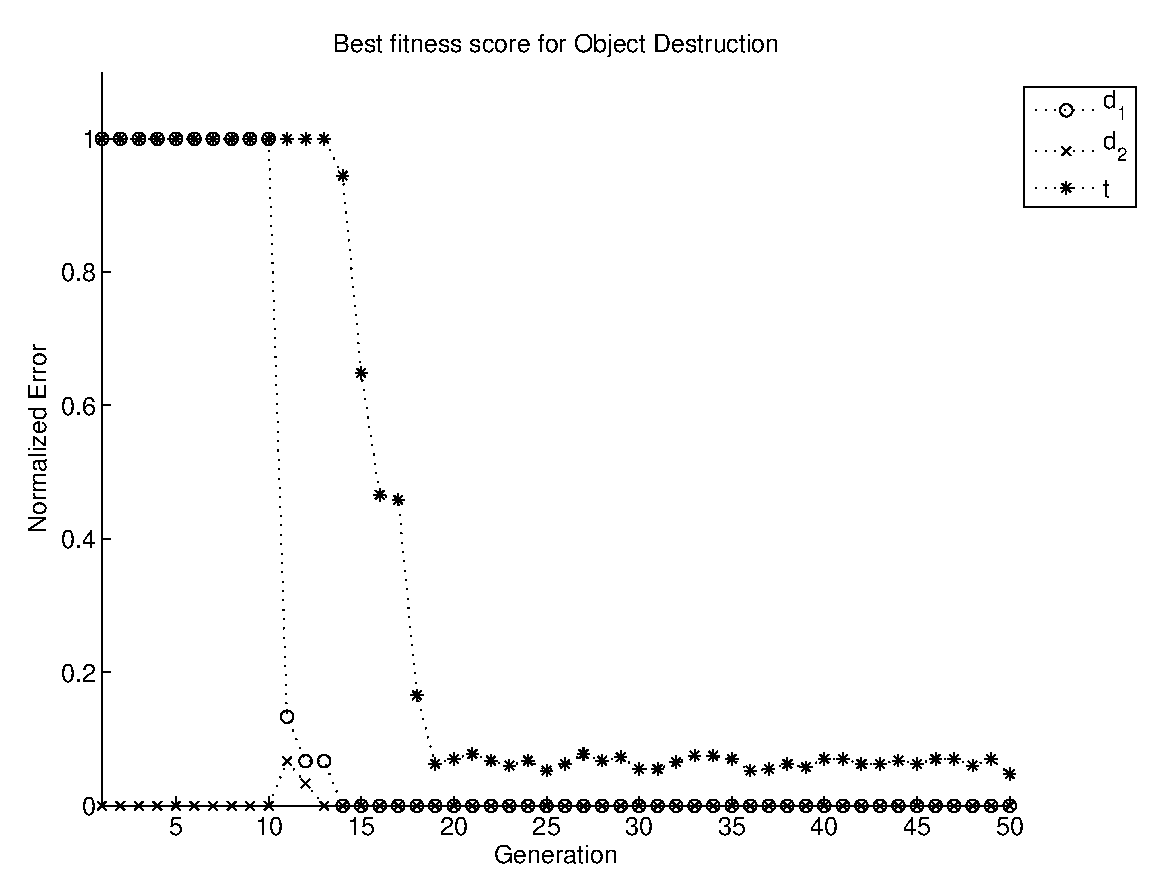
\includegraphics[height=.4\textheight]{ObjectDestructionBest}
  \caption[Progress of the best solution over 50 generations for object destruction.]{Progress of the best solution over 50 generations for object destruction is shown.  In generation 14, a solution that maximizes the fitness measures $d_1$ and $d_2$ is found.  Around generation 19, a more time-optimized solution to the object destruction problem is found.}
  \label{fig:DestructionBest}

  \vspace{.02\textheight}

  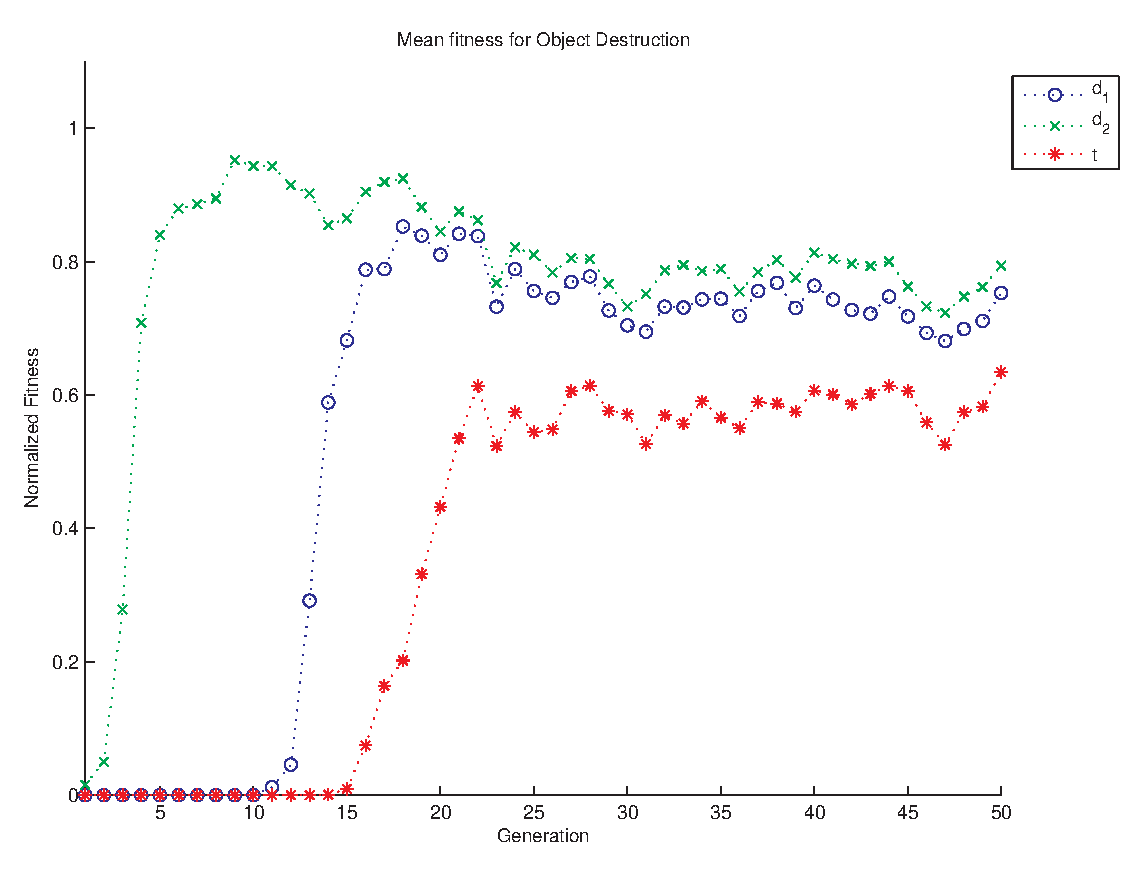
\includegraphics[height=.4\textheight]{ObjectDestructionMean}
  \caption[Mean fitness over time for object destruction.]{Mean fitness over time for object destruction is shown.  Notice how the mean fitness begins to decrease as soon as the best solution is found at generation 19.  This is attributed to the mutations being applied during reproduction since at this point most of the solutions in the population maximize $d_1$ and $d_2$, thus the probability that a random mutation will be helpful is small.}
  \label{fig:DestructionMean}
\end{figure}

\clearpage

%%%%%%%%%%
%%%%%%%%%%
%%%%%%%%%%

\subsubsection{Object Collection}

Over 8 separate evolutions, the average number of generations required to evolve a solution for object collection is approximately 55 generations. As seen in \refFigure{CollectionBest}, within 5 generation a solution is found that completely maximizes $c_2$, and within 10 generations a majority of the population is able to almost completely maximize $c_2$, as shown by \refFigure{CollectionMean}.  As the population drives towards maximizing $c_2$, slow progress is eventually made towards the maximization of $c_1$.  Mutated solutions that begin to maximize $c_1$ rise to the top of the fitness scale, thus being selected more often for reproduction.  Eventually in generation 21 a solution is produced that completely maximized $c_1$ and $c_2$.  As the population converges towards a set of complete solutions, the last metric to be addressed is the time $t$.  The performance of the best solution with respect to $t$ up until generation 45 is quite varied, indicating that the solutions are still relying on some form of serendipity to complete the task.  As seen in \refFigure{CollectionBest}, after generation 45, four marked periods of consistent performance occur.  During these periods, a single solution dominates the population, thus this one solution receives a majority of the mutations.  Hence at this point, the optimization of $t$ has essentially become a pure random search, using the mutation operators to explore the solution space around the best solution.  The additional work required to optimize $t$ is due to the fact that agents do not receive credit for navigating to the object repository unless they arrive there and successfully deposit the object they are holding.  Additionally, similar to what is seen in evolving object destruction, the mean fitness for the population increases once a complete solution is found.  

The solution evolved for object collection is shown in \refTable{CollectionAlgorithm}, and a simplified version of the algorithm is shown in \refTable{CollectionAlgorithmReduced}.  The simplifications include the removal of unreachable states and non-firing transitions, and the removal of actions that will have no effect.  

When executing the solution in \refTable{CollectionAlgorithmReduced}, each agent starts in state $A$.  No agent is holding any type $C$ objects at the beginning, so the second transitions in state $A$ cannot fire.  Thus the first time through state $A$, the agent eventually will select the first transition, attempt to pick up and object, and goto state $E$.  When transitioning from state $A$, the first two transitions in state $E$ cannot fire, but either the third or fourth will definitely be activated.  These two branches will be discussed separately.

First, if the agent is not near any type $C$ object, the third transition of state $E$ will fire, resulting in going to state $B$.  As a consequence of the transition to state $B$ from $E$, the first two transitions in state $B$ cannot fire.  If the agent is not holding a type $C$ object, the agent will transition to state $C$ and eventually end up back in state $A$.  If the agent is holding a type $C$ object, then the third transition in state $B$ fires, navigating the agent towards the goal area and transitioning into state $E$.  At this point, if the agent is in the goal area (which is unlikely), the agent will transition from state $E$ to state $G$, an inescapable loop that will cause the agent to hold onto the type $C$ object forever.  Now, in order for the agent to continue navigating towards the goal area, there cannot be any nearby objects preventing the firing of the third transition in state $E$.  If there is an object nearby, the agent will navigate towards it, broadcast its location, and wait to deliver its object until the other object is collected.  After cycling like this through states $B$ and $E$ until the agent is in state $B$ and located in the goal area, the first transition in state $B$ fires, and assuming that there are not type $C$ objects around, the agent will not move and will transition to state $A$, resulting in the completion of collecting one object.  Unfortunately, from here the agent transitions from $A \rightarrow F \rightarrow E \rightarrow G$.  Thus, after successfully collecting an object, the agent becomes useless as it is stuck in the infinite loop at $G$. 

The other branch point initially reached at state $E$ happens when the fourth transition fires because an agent is near an object.  The agent will cycle through states $E \rightarrow C \rightarrow A \rightarrow E$, navigating towards the object until it is picked up in state $A$.  At this point, the agent is holding an object and is in state $E$, which is the same situation previously discussed.

The evolved object collection algorithm does exhibit a form of emergent behavior.  Given the algorithm in \refTable{CollectionAlgorithmReduced} and a swarm of agents, the object collection task is performed quickly and completely.  But, when this algorithm is executed with only one or a few agents, the swarm fails to complete the object collection.  What happens is that an agent picks up an object in state $A$, transitions to state $E$, and if the agent is near any other objects, they navigate towards that object and broadcast its position until another agent picks up the object.  But in this case with one or few agents, there is no one able to collect the object and break the loop.  Thus, the agent(s) are locked in a broadcasting loop and never complete the object collection task.  

\clearpage

\begin{table}[ht]
  \centering
  \small
  \begin{tabular}{|c|c|l|c|}
    \hline
    State & Condition & Action & Next State \\
    \hline
    \input{FSA/collection.fsa}
  \end{tabular}
  \normalsize
  \caption{Evolved object collection algorithm}
  \label{tab:CollectionAlgorithm}
  
  \vspace{1cm}

  \small
  \begin{tabular}{|c|c|l|c|}
    \hline
    State & Condition & Action & Next State \\
    \hline
    \input{FSA/collection-reduced.fsa}
  \end{tabular}
  \normalsize
  \caption{Simplified version of the evolved object collection algorithm}
  \label{tab:CollectionAlgorithmReduced}
\end{table}

\begin{figure}[f]
  \centering

  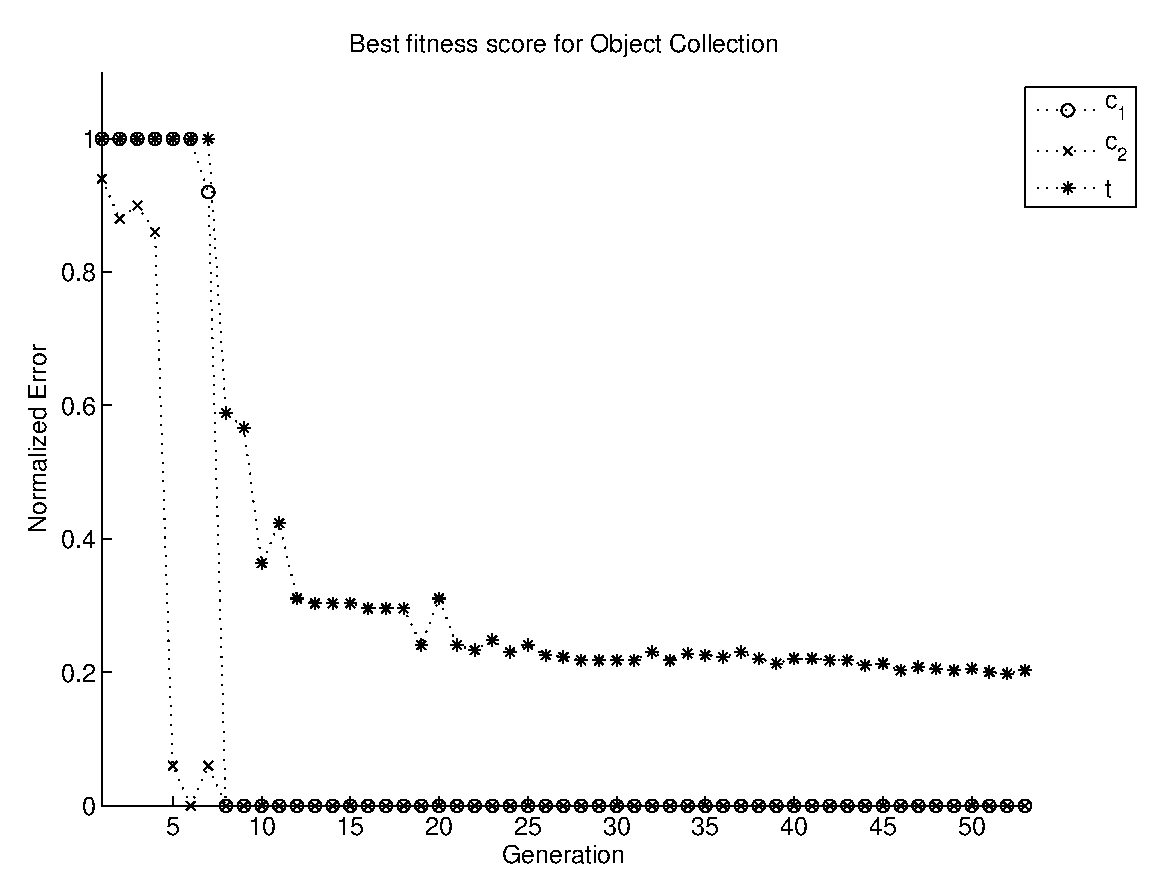
\includegraphics[height=.4\textheight]{ObjectCollectionBest}
  \caption[Progress of the best solution over time for object collection.]{Progress of the best solution over time for object collection is shown.  In generation 21, a solution that maximizes the fitness measures $c_1$ and $c_2$ is found.  Around generation 150, a time-optimized solution to the object collection problem is found.}
  \label{fig:CollectionBest}

  \vspace{.02\textheight}

  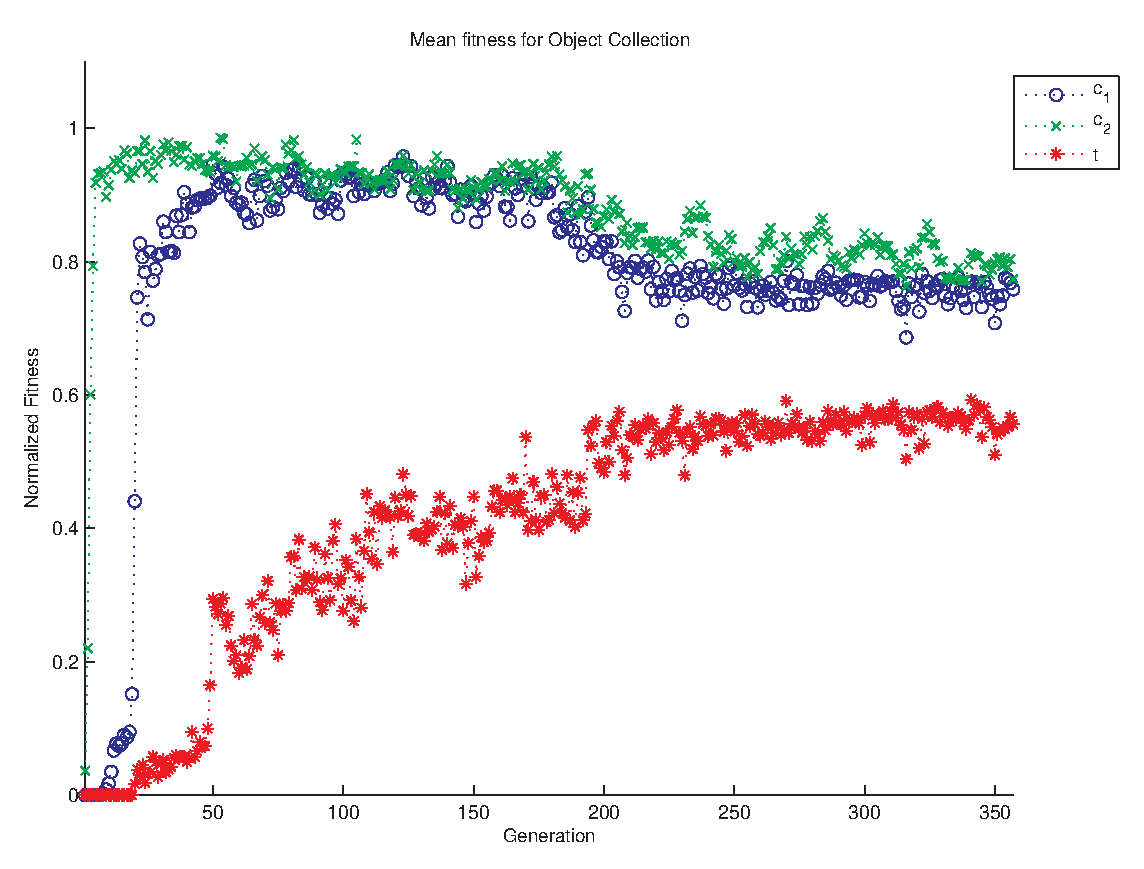
\includegraphics[height=.4\textheight]{ObjectCollectionMean}
  \caption[Mean mean fitness for object collection.]{Mean mean fitness over 350 generations for object collection is shown.  Notice how the mean fitness begins to decrease as soon a the best solution is found at generation 150.  This is attributed to the mutations being applied during reproduction since at this point most of the solutions in the population maximize $c_1$ and $c_2$, thus the probability that a random mutation will be helpful is small.}
  \label{fig:CollectionMean}
\end{figure} 

\clearpage

%%%%%%%%%%
%%%%%%%%%%
%%%%%%%%%%

\subsubsection{Object Manipulation}

The final scenario presented to the system is the complete object manipulation scenario involving the simultaneous collection and destruction of all the objects in the environment.  The average behavior of the evolution of an object manipulation solution is much less well defined than the behavior of either of the other scenarios.  As shown by \refFigure{ManipulationBest} and \refFigure{ManipulationBest2}, two different runs of object manipulation can have very different behavior with respect to convergence.  In \refFigure{ManipulationBest}, almost 325 generations are required to evolve a solution that completely collects and destroys all the objects in the environment, but only around 160 generations for the run shown in \refFigure{ManipulationBest2}.  Additionally, the best solution from the run shown in \refFigure{ManipulationBest} used 80\% of the allotted runtime, whereas the best solution from the run shown in \refFigure{ManipulationBest2} uses only 50\% of the allotted runtime. 

Over 8 different trials, evolving a solution for object manipulation required approximately 300 generations to find a complete solution, and at least 100 additional generations was required to begin time optimizing a solution.  The convergence time for the combined object collection and destruction scenarios is much longer than that of the individual scenarios.  This performance is expected as the multiple independent objectives compete with each other for survival.  

The balancing effect of the radix sorting can be seen in both \refFigure{ManipulationMean} and \refFigure{ManipulationMean2}, preventing one metric from dominating and skewing the mean performance of the population towards that metric.  This point is clearly illustrated through the progress of the mean population performance shown in \refFigure{ManipulationMean}.  Metrics $m_6$ and $m_8$, representing the secondary subtasks for object collection or destruction, and metrics $m_5$ and $m_7$, representing the completion of the object collection or destruction task, do not deviate far from each other.  Also notice the effect of the radix scoring and how neither of the two main tasks (collection or destruction) take a commanding lead over the other task.  Additionally, unlike the object collection and destruction evolutions, due to the larger search space the mean fitness does not begin to increase after a good solution is found.

The performance of the radix scoring is observed in \refFigure{ManipulationSum}; note how the number of solutions that satisfy one of the four metrics $m_1, m_2, m_3,$ or $m_4$ increases with respect to the progress made by the best solution.  This same performance can also be observed through \refFigure{ManipulationM5-second} and \refFigure{ManipulationM7-second}, which depict the complete progress of the population over time for metrics $m_5$ and $m_7$ respectively.  \refFigure{ManipulationM5-second} shows the fitness of every solution, indexed by generation, with respect to metric $m_5$.  So, for example, in generation 300, almost half the population has maximized $m_5$ to 1, a quarter of the population is very close to 1, and about 10\% of the population are not maximizing $m_5$ at all.  Similarly to \refFigure{ManipulationM5-second}, \refFigure{ManipulationM7-second} represents the fitness of all generations with respect to $m_7$.

Unlike the previous two scenarios, where once a complete solution is discovered that solution is further evolved for faster performance, no noticeable performance increases are guaranteed in this scenario once a complete solution is found, as shown in the difference between \refFigure{ManipulationBest} and \refFigure{ManipulationBest2}.  Overall, about 50\% of the time a complete solution is evolved that is able to perform quickly.  The inability of the system to consistently evolve a fast solution is attributed to the increased number of actions and sensor options in this scenario,  thus increasing the complexity of the evolved solution as compared to the previous evolved solutions, and exponentially increasing the number of candidate solutions.

The faster of the two solutions evolved for object collection is shown in \refTable{ManipulationAlgorithm}, and a simplified version of the algorithm is shown in \refTable{ManipulationAlgorithmReduced}.  The simplifications include the removal of unreachable states and non-firing transitions, and the removal of actions that will have no effect.  

The solution evolved here is much more complex than either of the solutions evolved for object collection or object destruction.   For the most part, the main functionality of the solution is spread across multiple states.  Due to the complexity of the solution and distribution of functionality across many states, it is difficult to analyze the algorithm completely and extract core behaviors.  With this in mind, a brief analysis of the salient portions of the algorithm will be discussed.

If an agent is in state $A$ and is on a type $C$ object, the agent will pick up the object and transition to state $J$.  Given a typical run of events, the agent will navigate to the goal area and deposit the object, cycling through states $J \rightarrow G \rightarrow K \rightarrow J$.  

If an agent is not on a type $C$ object, they will loop through state $A$ until they are near some type of object.  Upon sensing a type $C$ object, the agent transitions to state $J$.  From here, most likely they will fire the last transition in state $J$, which leads to state $I$, and begin to navigate towards the nearest type $C$ object.  From state $I$ the agent will most likely transition to state $C$ where it will loop until one of the conditions on the transitions is met.  At this point, the serendipity of the agent's random walk is relied upon to guide the agent towards the type $C$ object.  If the agent does in fact get to the object, the agent will broadcast the location of the object, transition to state $J$ and then to state $A$, where it will pick up the object.  From this point, the agent will deliver the object to the goal area as previously discussed.

In the other case, if the agent starting in state $A$ wanders until it is in the proximity of a type $D$ object, the agent transitions to state $H$, broadcasts the location of the object, and then transitions to state $G$.  From state $G$, it is difficult to reason about what transition an agent will follow because there are many possible situations.  In examining simulation runs with only a single agent, the basic result is that the agent will essentially rely on serendipity to guide the final steps towards the object, then most likely the object will be acted on in state $F$ reached through state $I$.

\section{Conclusion}

In this chapter, swarm algorithms have been successfully evolved for agent dispersion, object collection, and object destruction.  Composite fitness metrics, created through the fusion of raw fitness data, and a radix-based ranking algorithm were used to address the multi-objective nature of the object manipulation problem.  In evolving the object collection and object destruction algorithms, first the core functionality (collection and destruction, respectively) was evolved.  Then, evolution continued and optimized for execution speed.  The object manipulation scenario followed this trend of first evolving core functionalities, then optimizing for speed.  But unlike the evolution of the object collection and destruction algorithms, the complexity of the object manipulation problem prevented the consistent evolution of an algorithm that performed the object manipulation task quickly.

\begin{table}[ht]
  \centering
  \caption{Evolved object manipulation algorithm}
  \small
  \begin{tabular}{|c|c|l|c|}
    \hline
    State & Condition & Action & Next State \\
    \hline
    \input{FSA/manipulation.fsa}
  \end{tabular}
  \label{tab:ManipulationAlgorithm}
\end{table}

\begin{table}[ht]
  \centering
  \caption{Simplified version of the evolved object manipulation algorithm}
  \small
  \begin{tabular}{|c|c|l|c|}
    \hline
    State & Condition & Action & Next State \\
    \hline
    \input{FSA/manipulation-reduced.fsa}
  \end{tabular}
  \label{tab:ManipulationAlgorithmReduced}
\end{table}

\begin{figure}[f]
  \centering
  %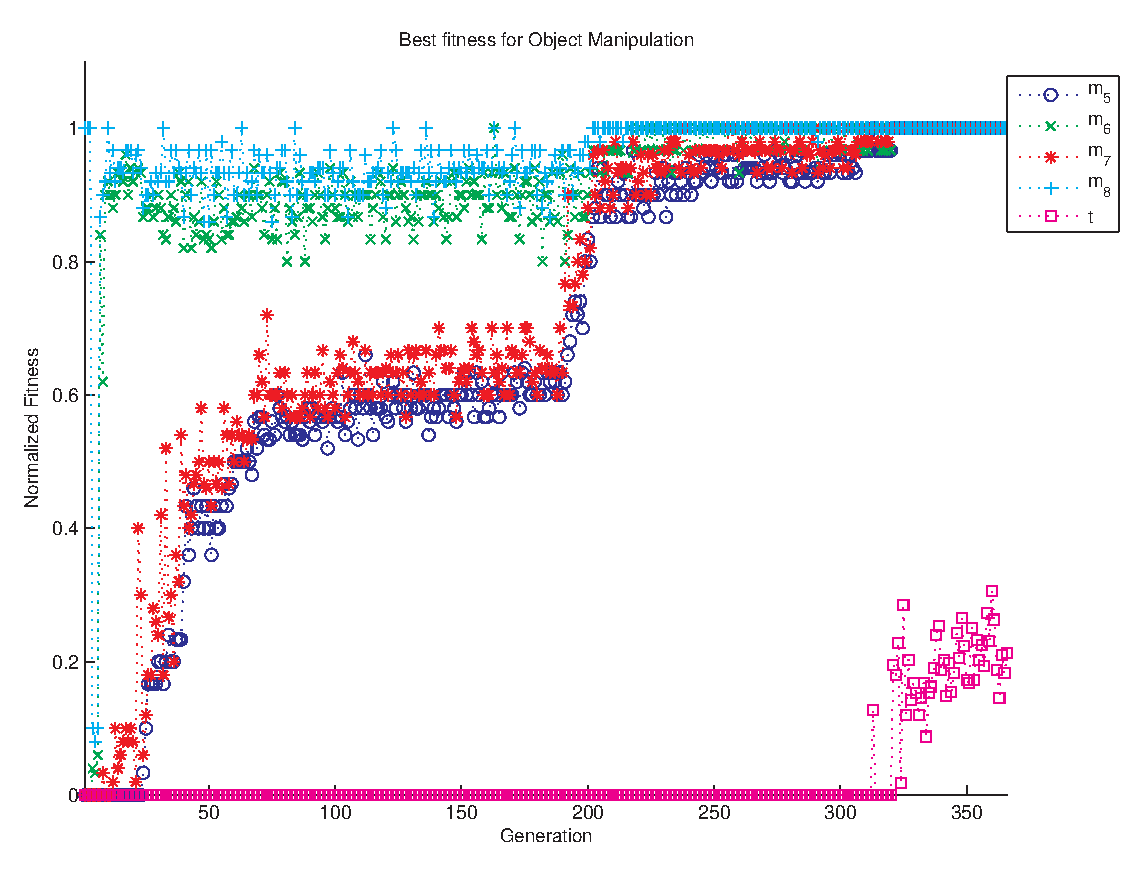
\includegraphics[width=.9\textwidth]{ObjectManipulationBest-1}
  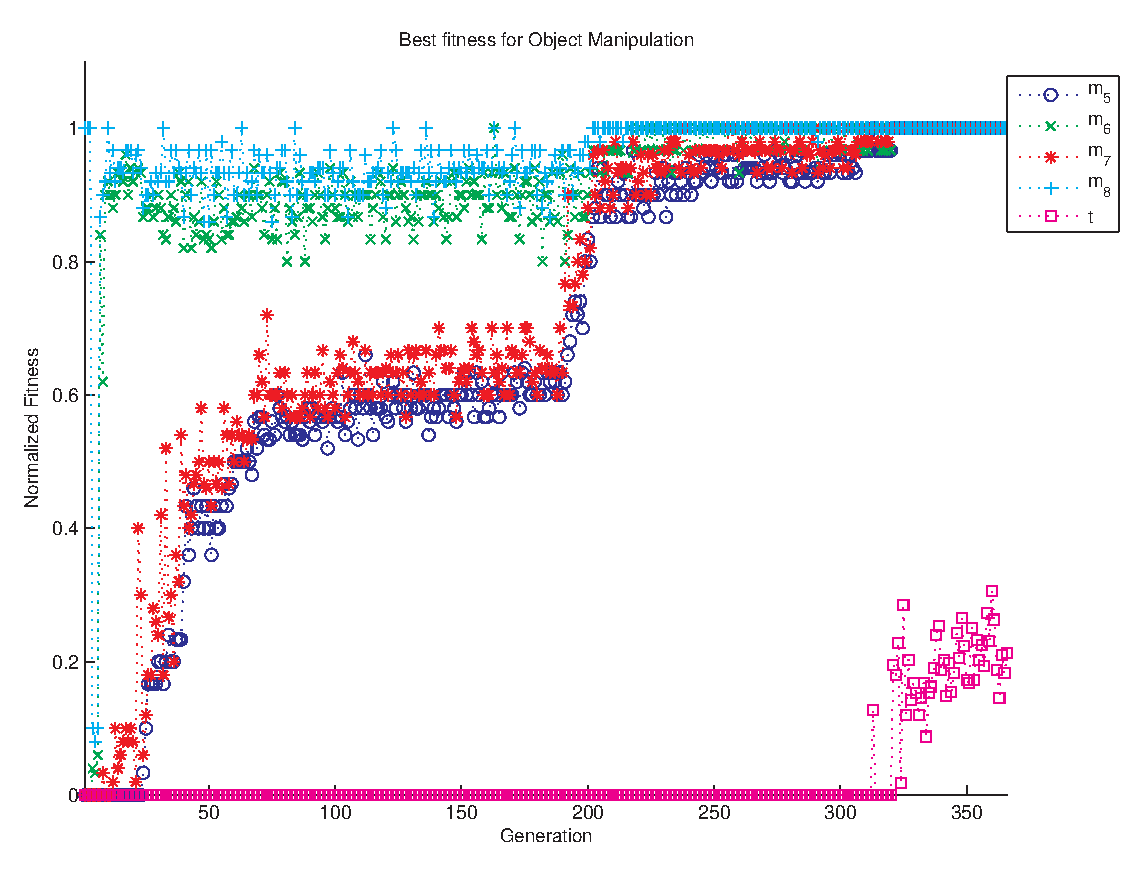
\includegraphics[height=.4\textheight]{ObjectManipulationBest-1}
  \caption[Progress of the best solution for object manipulation.]{Progress of the best solution over 360 generations for object manipulation is shown.  In generation 325, a solution that maximizes the fitness measures $m_5$--$m_8$ is found.  After this, some progress is made on optimizing the speed of the algorithm, but no real progress is made.}
  \label{fig:ManipulationBest}
%\end{figure}
%\hfill
%\begin{figure}[f]
%  \centering
  %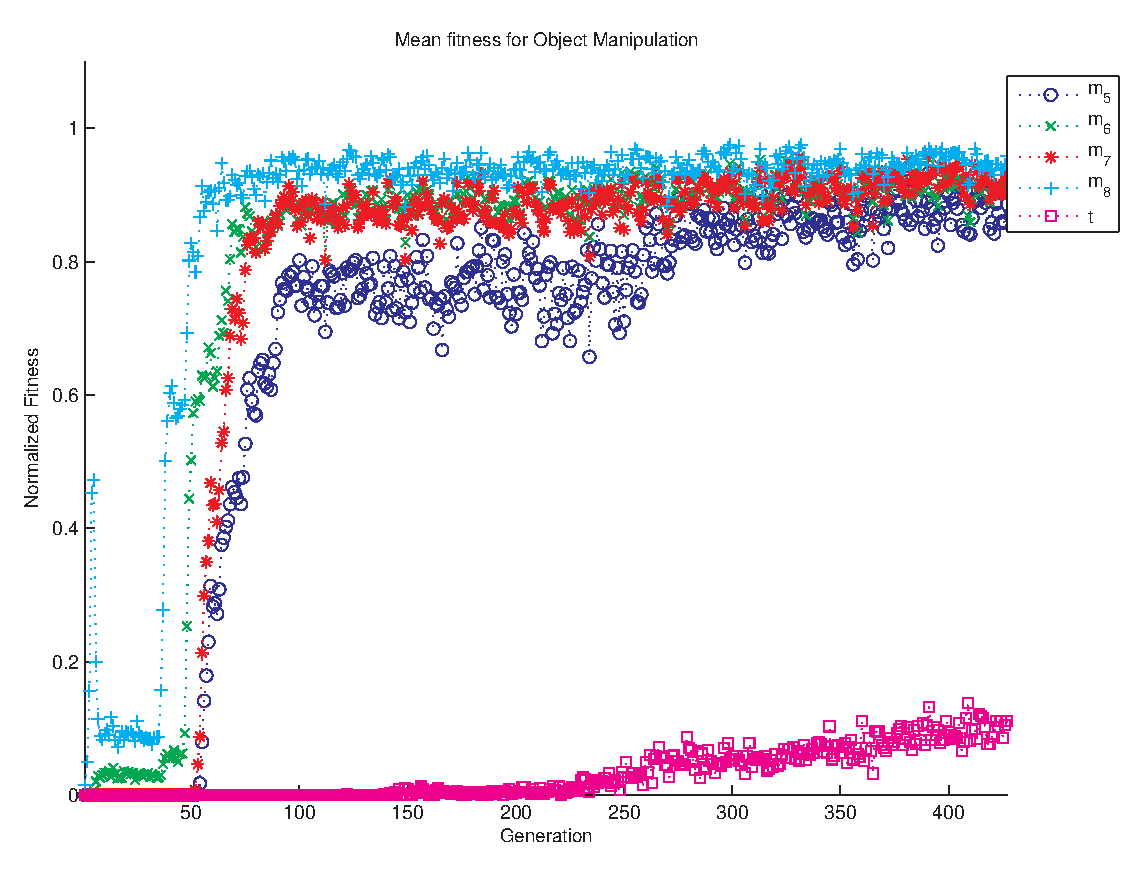
\includegraphics[width=.9\textwidth]{ObjectManipulationMean-2}
  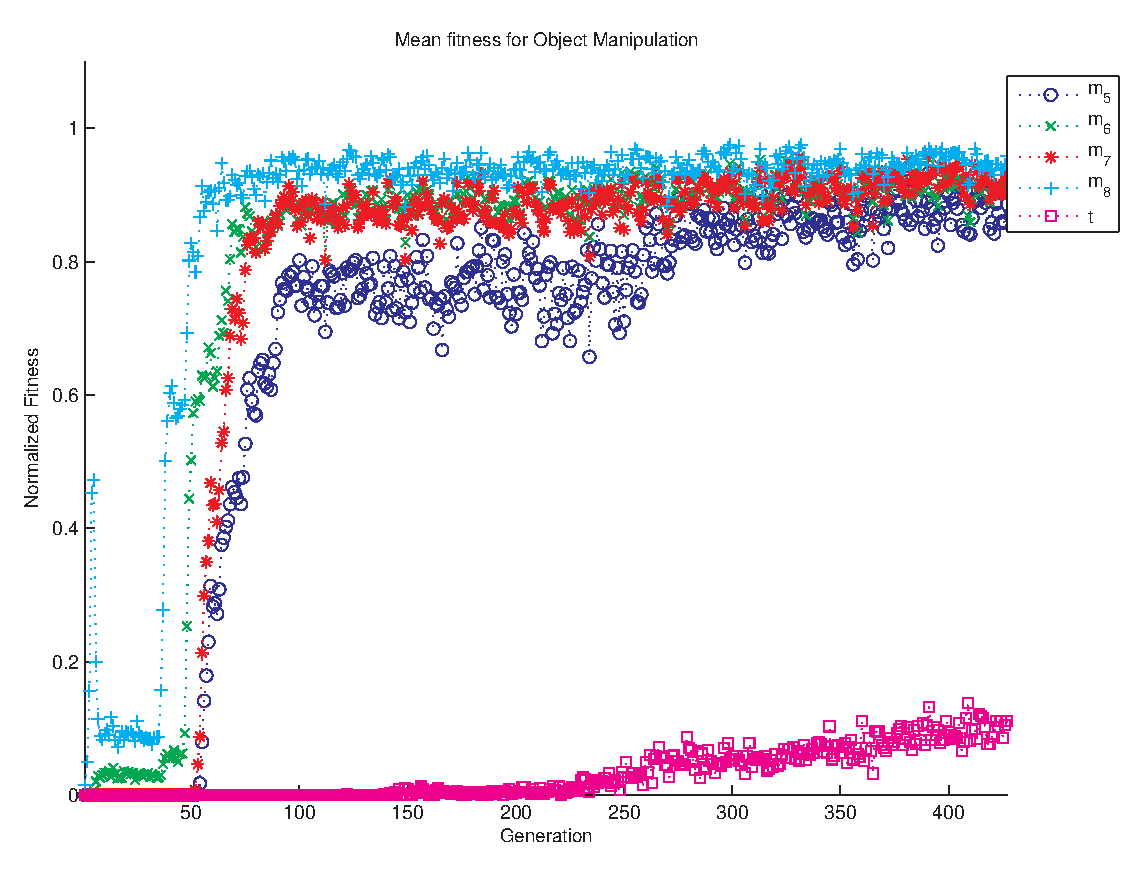
\includegraphics[height=.4\textheight]{ObjectManipulationMean-2}
  \caption[Mean fitness over time for object manipulation.]{Mean fitness over time for object manipulation is shown.  Notice the effect of the radix scoring and how neither of the two main tasks (collection or destruction) take a commanding lead over the other task.  Also, unlike the object collection and destruction evolutions, due to the larger search space, the mean fitness does not begin to decrease after a good solution is found.}
  \label{fig:ManipulationMean}
\end{figure}

\begin{figure}[f]
  \centering
  %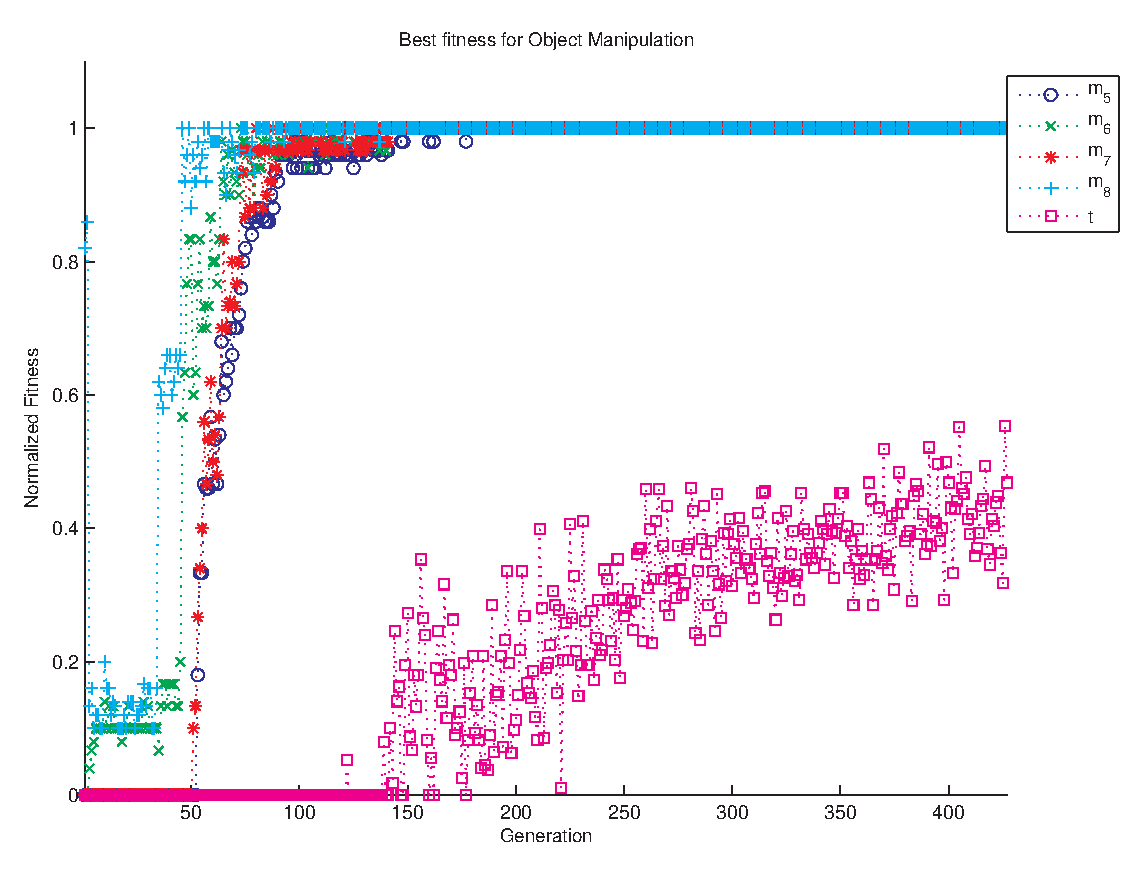
\includegraphics[width=.9\textwidth]{ObjectManipulationBest-2}
  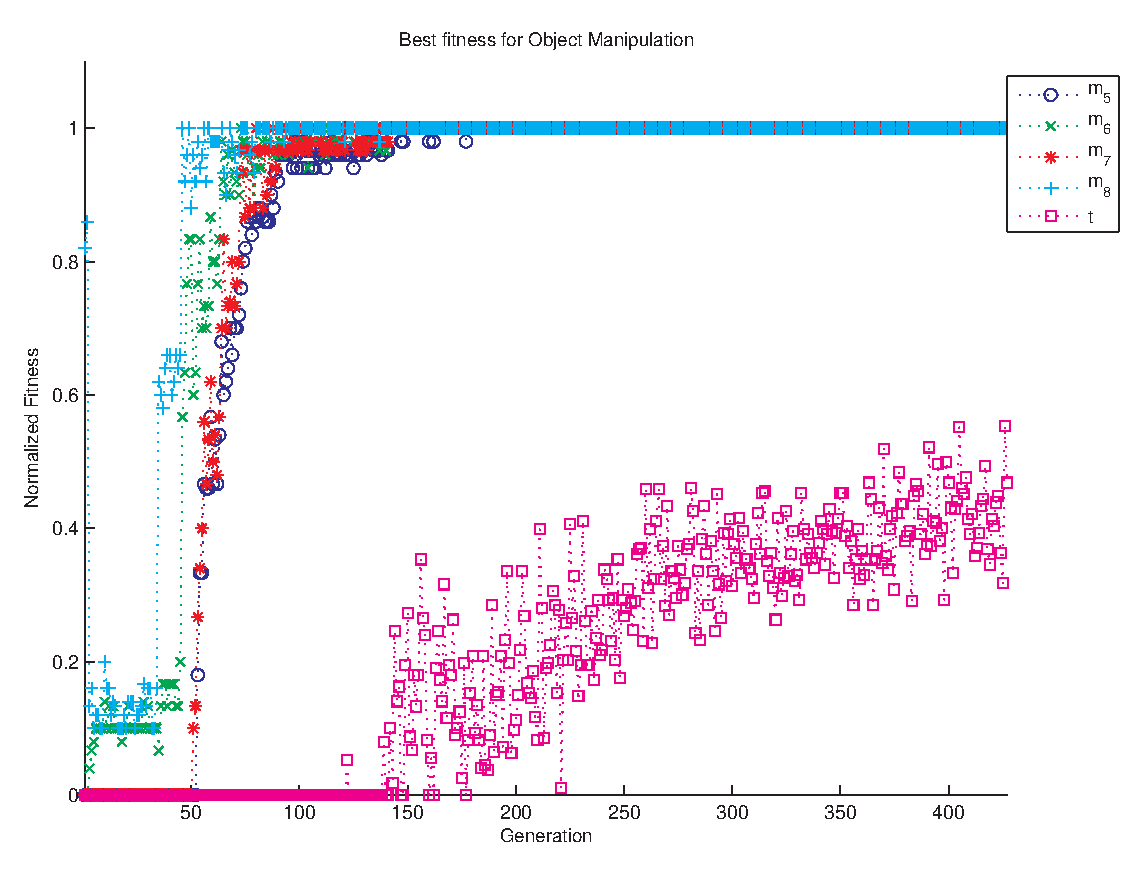
\includegraphics[height=.4\textheight]{ObjectManipulationBest-2}
  \caption[Progress of the best solution for another object manipulation evolution.]{Progress of the best solution over 425 generations for another object manipulation evolution is shown.  In generation 160, a solution that maximizes the fitness measures $m_5$--$m_8$ is found.  Around generation 160, a modest amount of progress in time optimization is achieved, resulting in a solution that is faster than the one evolved in \refFigure{ManipulationBest}.}
  \label{fig:ManipulationBest2}
%\end{figure}
%
%\begin{figure}[f]
%  \centering
%  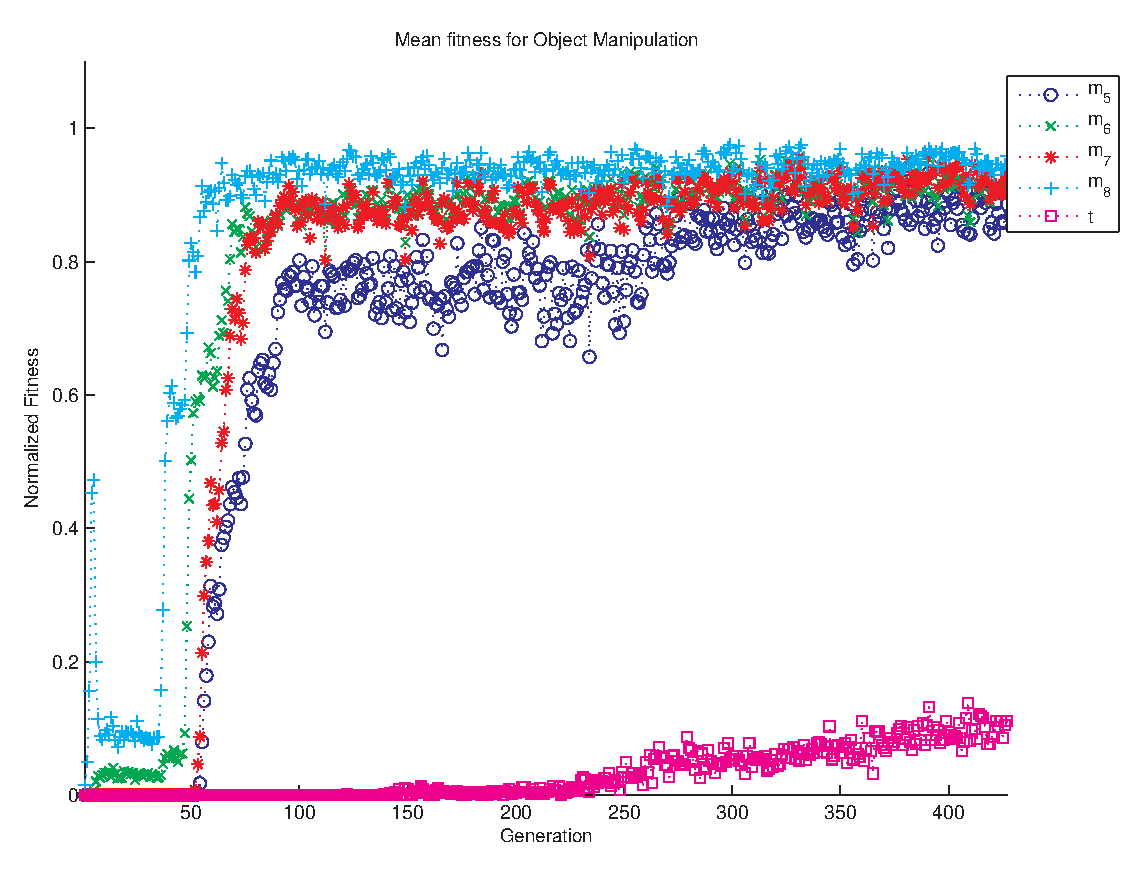
\includegraphics[width=.9\textwidth]{ObjectManipulationMean-2}
  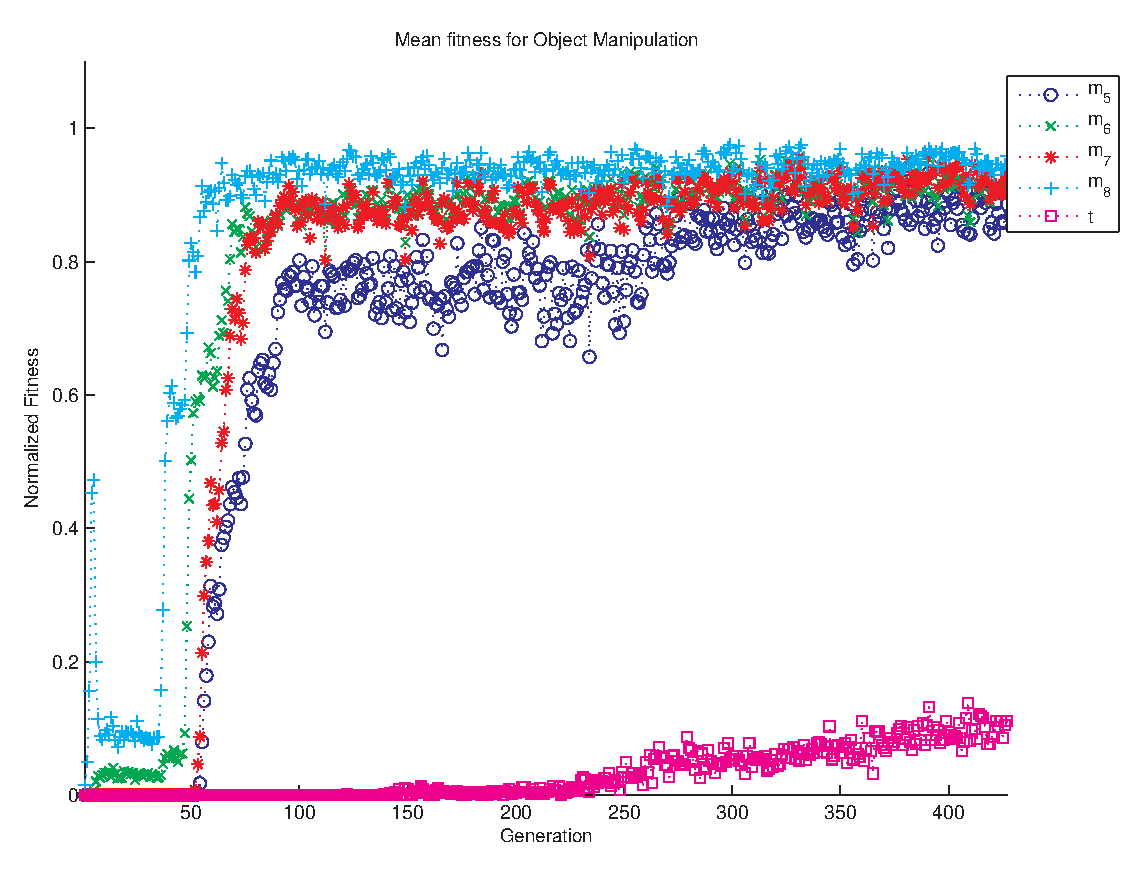
\includegraphics[height=.4\textheight]{ObjectManipulationMean-2}
  \caption[Mean fitness over time for the second object manipulation evolution.]{Mean fitness over time for the second object manipulation evolution is shown.  Again, notice the effect of the radix scoring and how neither of the two main tasks (collection or destruction) take a commanding lead over the other task.  Also, unlike the object collection and destruction evolutions, due to the larger search space, the mean fitness does not begin to decrease after a good solution is found.}
  \label{fig:ManipulationMean2}
\end{figure}

\begin{figure}[f]
  \centering

  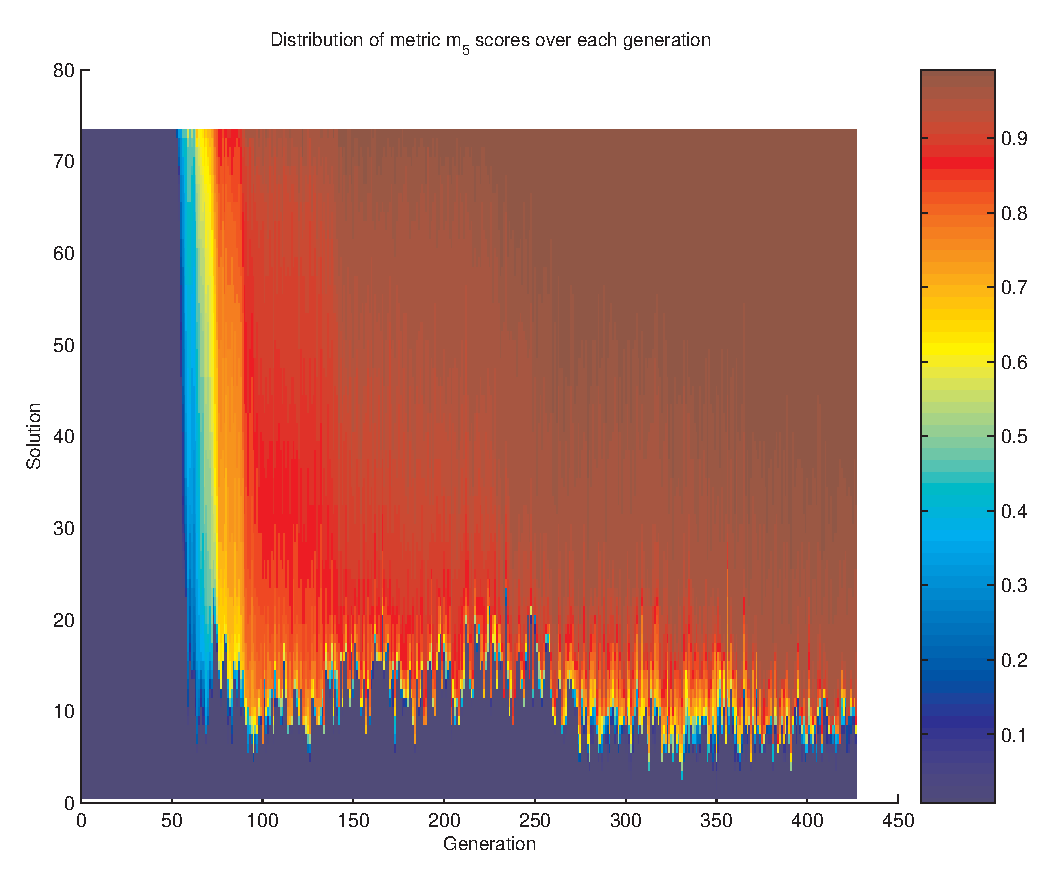
\includegraphics[height=.4\textheight]{ObjectManipulationM5-2}
  \caption{The fitness of every solution indexed by generation with respect to metric $m_5$.}
  \label{fig:ManipulationM5-second}

  \vspace{.05\textheight}

  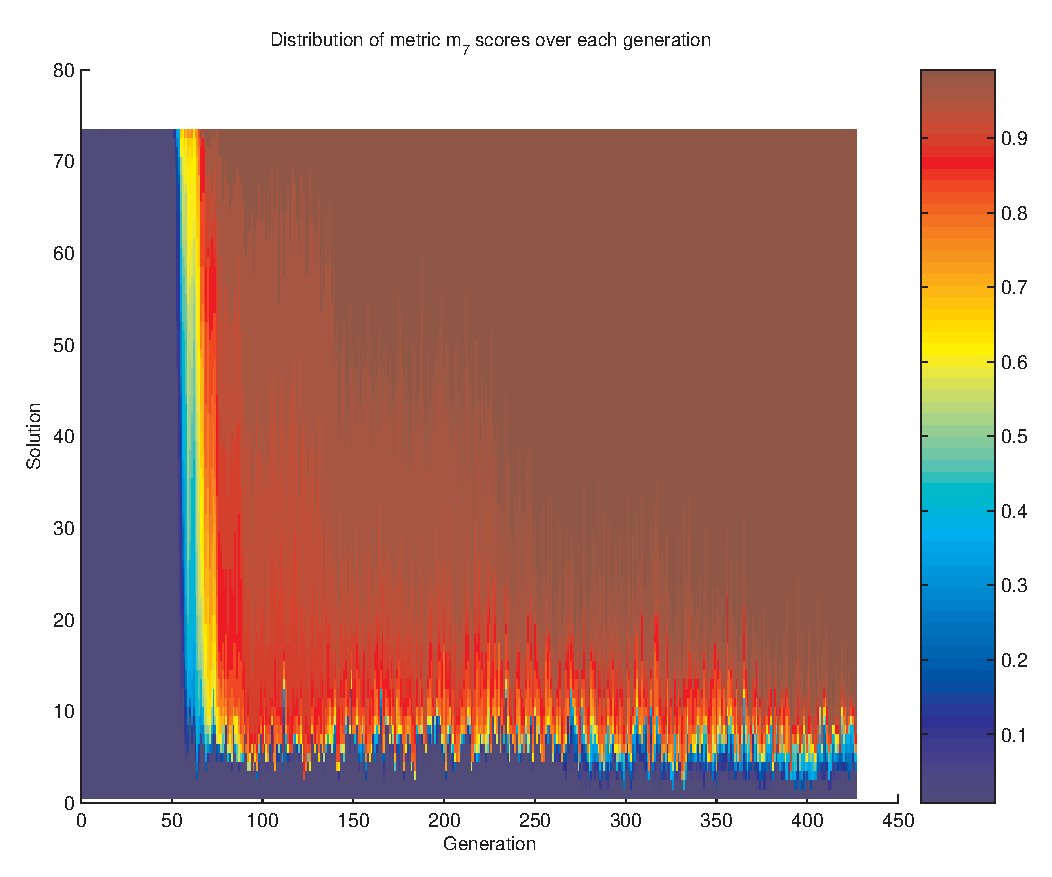
\includegraphics[height=.4\textheight]{ObjectManipulationM7-2}
  \caption{The fitness of every solution indexed by generation with respect to metric $m_7$.}
  \label{fig:ManipulationM7-second}
\end{figure}

\begin{figure}[f]
  \centering
  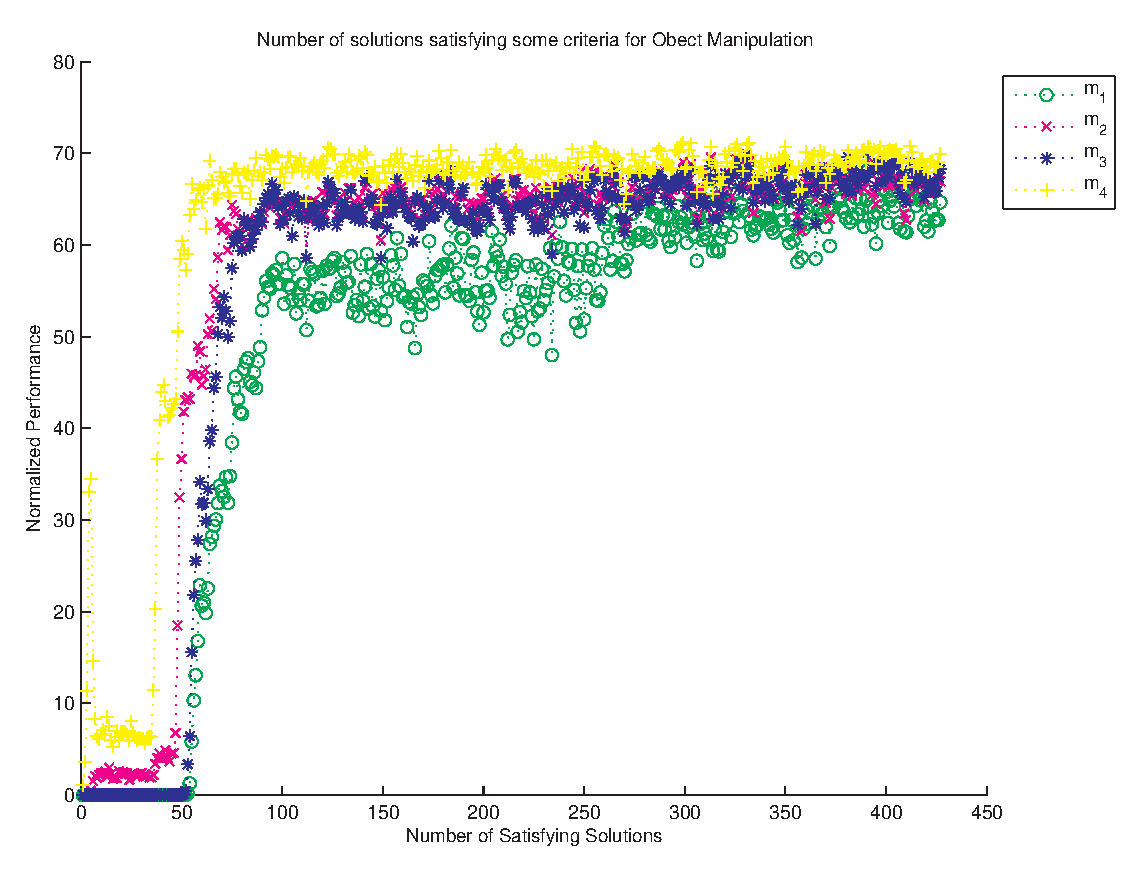
\includegraphics[scale=.7]{ObjectManipulationSum-2}
  \caption{Number of solutions satisfying criteria $m_1, m_2, m_3,$
    and $m_4$ for object manipulation.}
  \label{fig:ManipulationSum}
\end{figure}
